\documentclass[11 pt]{article}

\usepackage[utf8]{inputenc}
\usepackage[T1]{fontenc}
\usepackage[french]{babel}

\usepackage{amsmath}
\usepackage{empheq}
\usepackage{tikz}
\usepackage{tikz-qtree}
\usepackage{listings}
\usepackage{graphicx}
\usepackage{algorithm2e}
\usepackage[left=2cm,right=2cm,top=1.5cm,bottom=1.5cm]{geometry}
\usepackage[toc,page]{appendix}
\usepackage{hyperref}
\hypersetup{
  colorlinks,
  citecolor=black,
  filecolor=black,
  linkcolor=black,
  urlcolor=black
}

\title{Projet Transboost}
\author{Luc Blassel, Romain Gautron, Xue Bai, Yifei Fan, Xuefan Xu}

\begin{document}
\maketitle

\tableofcontents
\newpage

\section{Objectif et motivations}
\paragraph{}L’apprentissage supervisé  classique nécessite un grand nombre de données étiquetées, et dans certains cas une période de temps très importante, pour pouvoir établir des modèles fiables. Ceci n’est pas toujours possible dans le monde réel, parfois il n’est simplement pas possible de collecter assez de données pour entraîner nos modèles ou alors le temps necessaire pour l’entrainement du modèle est beaucoup trop long pour que ca soit pratique.  L’apprentissage par transfert peut nous aider à résoudre ce type de problèmes.

\paragraph{}L’apprentissage par transfert nous permet de transférer des connaissances apprises sur un domaine source, avec idéalement une grande quantité de données étiquetées de bonne qualité, sur un domaine cible. Cette approche permet de réutiliser des portions d’un modèle préalablement entrainer dans notre nouveau modèle et ainsi de gagner du temps. Cette méthode est considérée comme le prochain moteur de succès de l’apprentissage automatique après l’apprentissage supervisé.

\paragraph{}La méthode TransBoost, introduite par Antoine Cornuéjols et ses collègues, propose une implémentation de l’apprentissage par transfert différente de la norme.  Quand l’approche “classique” de l’apprentissage par transfert, adapte l'hypothèse développée sur le domaine source au domaine cible, TransBoost en prend le contrepied. En effet dans cette dernière, on apprend l'hypothèse sur le domaine source et on projette ensuite les points du domaine cible sur le domaine source pour utiliser directement l'hypothèse source sur les points projetés. La projection des points du domaine cible sur le domaine source se fait dans le cadre d'un algorithme de boosting, qui, grâce à plusieurs projecteurs faibles, permet d’obtenir un projecteur fort. Ce dernier permet alors d’utiliser l'hypothèse source pour classifier les points du domaine cible.

\paragraph{}Cette méthode a d’abord été testée sur la classification de series temporelles incompletes, et à été un franc succès, en ayant de bien meilleures performances que d’autres approches au même problème. Cependant, la classification d’images etant le metre etalon en ce moment, le but de ce projet est d’adapter la méthode TransBoost à la classification d’images en utilisant des réseaux de convolution profonds (deep CNN).


\section{Problematique}
\paragraph{}L’application de la méthode TransBoost a la classification d’images oblige à se poser quelques questions. D’une part la très grande dimensionnalité des images force a utiliser des methodes tres lourdes telles que les réseaux de convolution profonds. Il existe dans les librairies de machine learning telles que TensorFlow des réseaux pré-entraînés, mais quel modèle choisir, pourquoi? D’une autre part la projection des points du domaine cible peut poser problème. Le choix a été fait de modifier les premieres couches du reseau utiliser pour classifier les images du domaine source, cependant il faudra trouver les meilleurs hyperparamètres tel que  le nombre de couches a re-entrainer, pour obtenir des performances optimales.

\section{Approche}
\subsection{idee generale}
\begin{figure}
  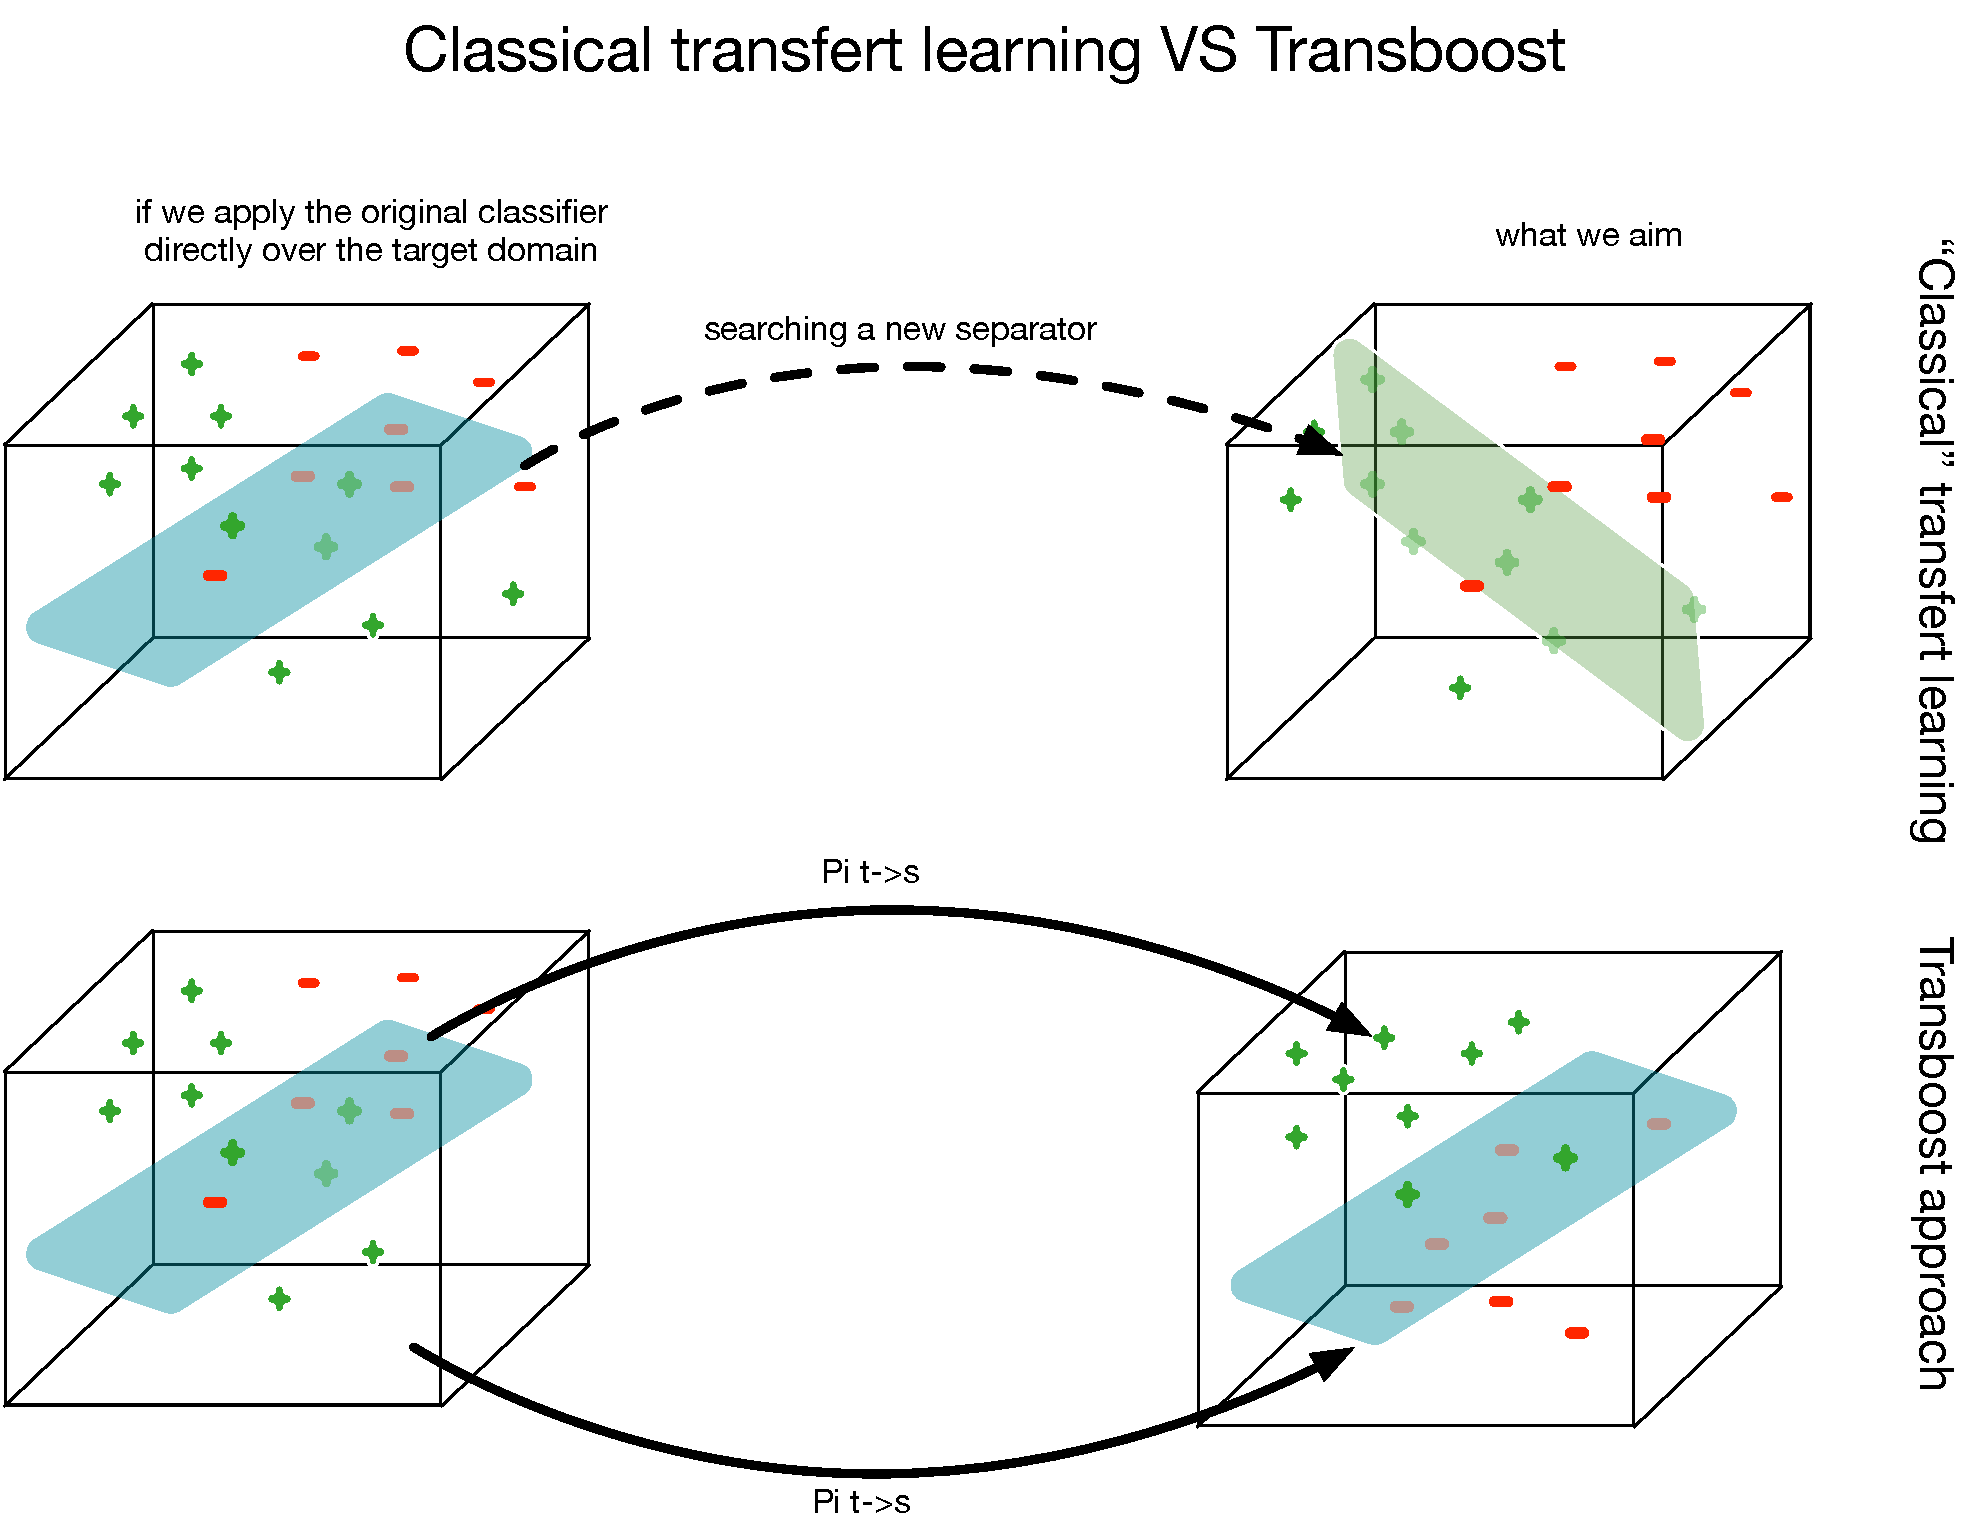
\includegraphics[width=\textwidth]{fig2.pdf}
  \caption{Differences entre l'approche classique et l'approche TransBoost}
  \label{figDiff}
\end{figure}


\paragraph{}Contrairement a l’apprentissage par transfert “classique”  il ne s’agit pas ici d’adapter l'hypothèse source au domaine cible, comme ce que l’on peut voir sur la première partie du schéma. Il faut donc projeter les points du domaine cible sur le domaine source avec une bonne précision pour que la séparatrice du classificateur source puisse différencier les images du domaine cible.\\
Cette méthode s’effectue de la manière suivante:\\ \medskip
\begin{itemize}
  \item on ajuste un CNN pre-entraine sur notre domaine source (avec 2 classes d’images) pour obtenir l'hypothèse source
  \item on gèle les n dernières couches du modèle et on ré-initialise les poids des premières couches
  \item on re-entraine le modèle partiellement gelé pour obtenir un projecteur/ classificateur.
\end{itemize}

\paragraph{}Dans le cas du boosting on effectue cette dernière étape de multiples fois pour obtenir des projecteurs faibles.

\paragraph{}Vu que les CNN disponibles ont souvent plus que deux classes de sortie, il est nécessaire de changer la couche de sortie du réseau et de l’entrainer pour l’ajuster a notre domaine source (binaire). Pour économiser du temps de calcul nous calculons les valeurs de transferts pour tous les points des jeux d’entrainement, de test et de validation du domaine source pour le réseau sans derniere couche. Ces valeurs de transferts sont alors utilisées pour entraîner la dernière couche séparément du réseau. Le réseau et la dernière couche sont alors unifiés pour former notre modèle source.

\paragraph{}Ce schema resume les etapes lors de l'application de cette methode:\\ \medskip

\begin{figure}
  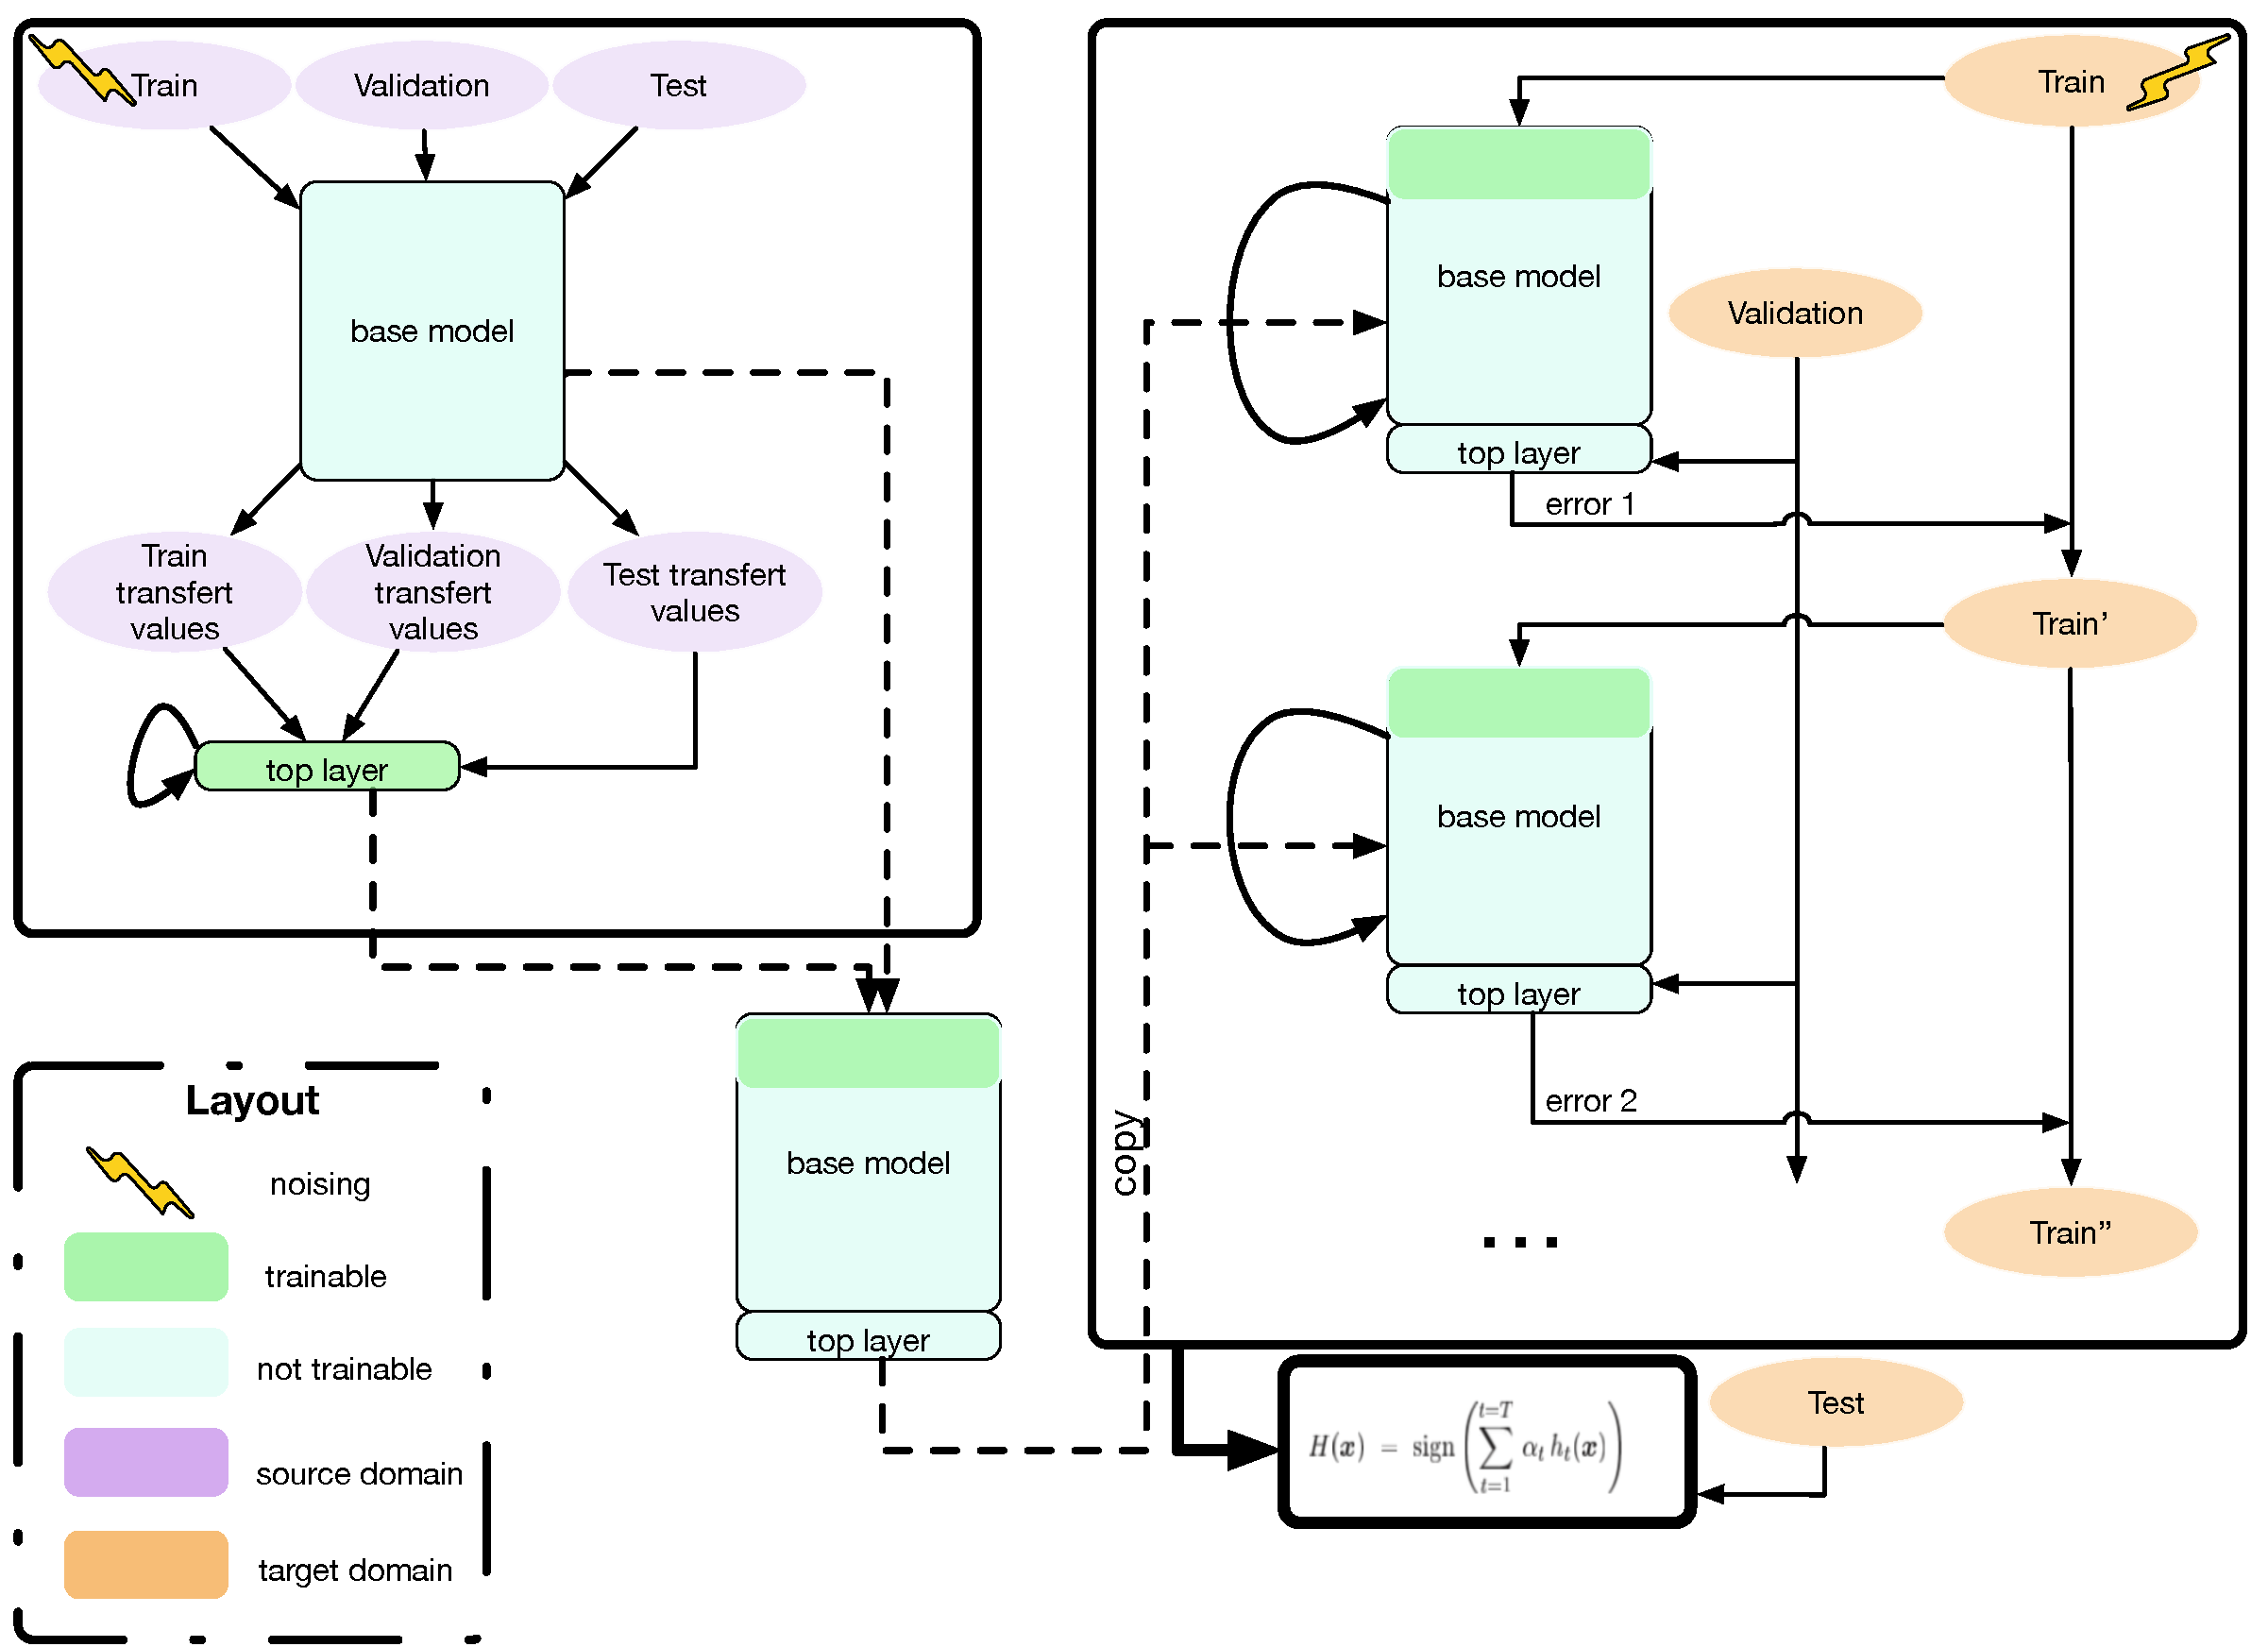
\includegraphics[width=\textwidth]{fig1.pdf}
  \caption{Deroulement de la methode TransBoost dans le cadre de ce projet}
  \label{figRes}
\end{figure}

\subsection{presentation des donnees}
\paragraph{}Nous avons choisis le data set CIFAR-10 composé d’images RGB 32x32. Celui-ci est composé de 60000 images se ventilant en 10 classes (avion,automobile,oiseau,chat,cerf,chien,grenouille,cheval,bateau,camion). Les motivations pour ce choix sont :\\ \medskip
\begin{itemize}
  \item qu’il s’agit d’un dataset de référence usuel dans le milieu
  \item que la faible de taille des images limite le volume des données à manipuler
  \item le faible nombre de classes permet néanmoins de constituer des couples plus ou moins ardus (avion/chat vs chien/chat)
\end{itemize}

\paragraph{}Les données sont déjà reparties en 3 ensembles : entrainement, validation et test. Pour pallier au faible nombre des données dans la base d’entraînement on introduira du bruit dans celles-ci pour éviter tout sur-apprentissage. Ce bruit consiste en des rotations, zooms, déformations aléatoires. Attention, aucun bruitage n’est appliqué aux ensemble de validation et de test. En effet, on veut ceux-ci les plus représentatifs possible des images “réelles” pour éprouver le modèle.

\paragraph{}Pour constituer les ensembles source et cible, il s’agit dans les faits de simple paramètres d’entrées qui permettent de changer les classes de manière aisée (exemple : classes\_source = ['dog','truck'], classes\_target = ['deer','horse']). A noter que le bruitage des sets d’entraînement est appliqué pour les deux domaines.

\subsection{Construction d'un classifieur binaire fort sur le domaine source}
\paragraph{}Afin de pouvoir mettre en application l’idée du TransBoost, nous devons tout d’abord obtenir un classifieur binaire fort sur une tâche et aussi bon que le hasard sur une seconde. Pour cela, nous devons d’abord choisir quel sera notre modèle de base. On entend par modèle de base un réseau profond déjà entraîné et sans les dernières couches (couches connectées et softmax). Keras offre de nombreuses possibilités de modèles (voir \href{https://keras.io/applications/}{ce lien}). Le choix s’est porté sur le modèle Xception, d’une part pour la qualité des valeurs de transferts qu’il produit et d’autre part pour le temps qu’il faut pour générer ces valeurs de transfert. On appelle valeurs de transfert les valeurs des fonctions d’activation de la dernière couche du modèle de base pour un ensemble d’images.

\paragraph{}Par soucis de parcimonie en temps de calcul, on fait passer l’ensemble des sets d’images dans le modèle de base une seule fois. On génère ainsi les valeurs de transfert qui serviront à l’entraînement de la dernière couche. \\
L’architecture de la dernière couche (plus exactement du dernier bloc) est :\\ \medskip
\begin{itemize}
  \item une couche entièrement connectée de taille 1024, activation “relu”
  \item un dropout à 50 \%
  \item une couche entièrement connectée de taille 512, activation “relu”
  \item un dropout à 50 \%
  \item un couche de taille 1, activation “sigmoid”
\end{itemize}

\paragraph{}Le choix de celle-ci s’est fait de manière empirique.\\
Comme pour le bruitage des images, le dropout est ici pour prévenir le surapprentissage compte tenu du faible nombre d’images présentées.
Une fois la dernière couche entraînée et répondant aux caractéristiques désirées, on assemble le modèle de base et ladite dernière couche en un modèle complet.


\subsection{Mise en pratique du TransBoost}
\paragraph{}Une fois que nous avons constitué notre classifieur fort, il faut voir la suite comme l’application classique d’Adaboost. La seule nuance est que, au lieu de repartir d’un classifieur “from scratch” on va cette fois partir d’un classifieur partiellement entraîné pour constituer notre projecteur faible.

\paragraph{}On cherche, non pas comme dans le transfert learning classique avec les CNN à réapprendre une nouvelle séparatrice linéaire en entraînant la dernière couche pour une nouvelle tâche. On cherche à faire rentrer pour la nouvelle tâche les points des bons cotés de la séparatrice pour la tâche précédente en cherchant des descripteurs de faibles niveau correspondants (i.e. en ré-entraînant les premiers blocs du réseaux de neurones profond) pour que cela soit réalisé.

\paragraph{}Pour ce faire,  on prend le modèle que nous avions à l’étape précédente, on dégèle les premières couches du modèle de base et on gèle tout le reste. A ce stade deux approches sont possibles : soit réinitialiser les poids des couches dégelées soit conserver les poids. Il se peut qu’en réinitialisant le poids de ces couches avec des descripteurs de faible niveau ne permette pas à l’algorithme de converger sur si peu de données. La réponse viendra des expérimentations. Dans les deux cas, le modèle résultant de l’étape citée servira de classifieur à entraîner lors des étapes de boosting.\\
Trois paramètres importants sont à chercher selon un compromis performances/coût calculatoire :\\ \medskip
\begin{itemize}
  \item la force des classifieurs (seuil de précision) à chaque étape de boosting
  \item le nombre de blocs convolutifs à entraîner
  \item le nombre de projecteurs faibles entraînés
\end{itemize}

\paragraph{}La suite est celle de l’algorithme Adaboost. A noter que l’erreur totale du modèle est mesurée sur le set de validation. Par contre le modèle est bien entraîné sur le set d’entraînement pondéré, et la pondération des points basée sur les prédictions faites sur ledit set d’entraînement.\\
A chaque étape, l’entraînement d’un projecteur s’arrête lorsqu’un seuil de précision est atteint (avec une limite d’un grand nombre d’epochs).

\begin{algorithm}
  \SetAlCapSkip{10ex}
  \SetKwInOut{Input}{input}\SetKwInOut{Output}{output}
  \SetKw{Init}{Initialisation:}
  \Input{$\mathcal{X_S}\rightarrow\mathcal{Y_S}$ :  l'hypothese source\\
          $\mathcal{S_T = \{(X_i^T,Y_I^T)\}}_{1\leq i\leq m}$ : l'ensemble d'entrainement cible}
  \Init{} de la distribution sur le jeu d'entrainement:$D_1(i)=1/m\ for\ i=1,\cdots,m$\;
  \For{$n=1,\cdots,N$}{
    Trouver une projection $\pi_i:\mathcal{X_T\rightarrow X_S}$ tq. $h_S(\pi_i(.))$ soit meilleure que le hasard sur $D_n(\mathcal{S_T})$\;
    Soit $\epsilon_n$ le taux d'erreur de $h_S(\pi_i(.))$ sur $D_n(\mathcal{S_T})$: $\epsilon_n = P_{i~D_n}[h_S(\pi_n(x_i))\neq y_i]$(avec $\epsilon_n<0.5$)\;
    Calculer $\alpha_i=\frac{1}{2}log_2(\frac{1-\epsilon_i}{\epsilon_i})$\;
    Mettre a jour: \For{$i=1,\cdots,m$}{
        \begin{equation*}
          \begin{split}
            D_{n+1}(i) & = \frac{D_n(i)}{Z_n}\times\begin{cases}
              e^{-\alpha_n}\ si\ h_{\mathcal{S}}(\pi_n(x_i^{\mathcal{T}}))=y_i^{\mathcal{T}} \\
              e^{\alpha_n}\ si\ h_{\mathcal{S}}(\pi_n(x_i^{\mathcal{T}}))\neq y_i^{\mathcal{T}}
            \end{cases}\\
            & = \frac{D_n(i)exp(-\alpha_n y_i^{(\mathcal{T})}h_{\mathcal{S}}(\pi_n(x^{(\mathcal{T})})))}{Z_n}
          \end{split}
        \end{equation*}
        Ou $Z_n$ est un facteur de normalisation tq. $D_{n+1}$ soit une distribution de $\mathcal{S_T}$\;
    }
  }
  \Output{L'hypothese finale $H_{\mathcal{T}}:\mathcal{X_T \rightarrow Y_T}$:\\
            $ H_{\mathcal{T}}(x_{\mathcal{T}})=signe\{\sum\limits_{n=1}^N \alpha_n h_{\mathcal{S}}(\pi_n(x^{\mathcal{T}}))\}$}

  \caption{Algorithme Transboost}
\end{algorithm}

\subsection{Comparaisons critiques portant sur la methode transboost}
\subsubsection{Projecteurs faibles vs. projecteurs forts}
\paragraph{}On veut comparer l’approche TransBoost avec faisant varier la force des projecteurs aux extrêmes. Si l’on obtient des performance supérieures avec un seul projecteur fort (i.e. les premiers groupes de couches convolutives entraînées aux maximum) alors on ne peut pas montrer un intérêt de travailler avec une multitudes de projecteurs faibles en boosting dans ce cadre précis.

\subsubsection{Projecteurs vs. nouveau classifieur}
\paragraph{}Comme on le voit, la méthode du TransBoost appliquée avec le modèle complet (base et dernier bloc) est très gourmande en temps et en espace. En effet, après avoir entraîné un grand nombre de classifieurs il faut également stocker tous ceux-ci à fin de pouvoir réaliser les classification de nouveau points selon l’hypothèse finale. En fait, on peut être plus économe en espace. En effet, il suffit de la connaissance pour reconstruire tous les modèles issus du boosting :\\ \medskip
\begin{itemize}
  \item du modèle complet non modifié
  \item uniquement pour chaque étape de boosting du poids des couches modifiées
\end{itemize}
\paragraph{}On souhaite mettre en compétitions deux approches : le TransBoost et une méthode de boosting classique.

\paragraph{}On peut atteindre un seuil de précision relativement bas à chaque étape ( de l’ordre de 0.7) simplement à l’aide d’un petit réseau convolutif initialisé (quelques blocs). Bien qu’avec l’économie en espace citée précédemment il n’y ait pas beaucoup de différence, l’économie en temps de calcul est bien là. En effet pour chaque prédiction à faire, le passage dans le petit CNN suffit. Tandis qu’à chaque étape avec le modèle de base augmenté du dernier bloc il faille calculer les activations dans toute la partie supérieure gelée du réseau avant de "backpropager" l’erreur.


\subsection{Difficultes rencontrees}
\paragraph{}Nous avons fait la décision initiale de travailler dans un environnement purement Tensor Flow, puisque le modèle que nous avions choisi était disponible dans cette librairie. Cependant dès qu’il a ete temps de modifier la structure du modèle (pour avoir une couche de sortie binaire par exemple) ou qu’il a fallu geler l'entraînement de certaines couches l’utilisation de Tensor Flow est devenue tres compliquee. En effet l’objet du modele etait introuvable et il fallait modifier un graphe ce qui nous a posé beaucoup de problèmes. C’est pour cela que nous avons décidé d’utiliser la librairie keras qui fonctionne comme surcouche de Tensor Flow ce qui nous a permis d’utiliser les modèles disponible dans Tensor Flow mais en ayant des outils et une syntaxe plus claire et plus simple d’utilisation, permettant des temps de développement beaucoup plus courts.

\paragraph{}Nous avons aussi rencontré beaucoup de problèmes de ressources machine, puisque les machines physiques et virtuelles auxquelles nous avions accès présentaient des performances limitées. Ceci a engendré des temps d'exécution se comptant en dizaine d’heures et même en jours dans certains cas et aboutissant souvent a des erreurs de mémoire. Il est donc nécessaire d’avoir accès à une machine performante qui nous permettra debugger le programme et le perfectionner sans attendre des periodes tres longues. 


\section{Resultats}
\subsection{Construction du classifieur binaire}
\paragraph{}Dans les faits, pour la base d’apprentissage “chien/camion”, l’algorithme arrive à 98.9\% de précision sur le set de test en seulement 2 epochs. D’un autre côté ce même modèle entraîné sur le dataset précédent a un précision de 50\% en prédiction sur le dataset “deer/horse”, ce qui répond bien à ce que l’on recherchait.

\subsection{Boosting classique sur petit CNN}
\paragraph{}Avec un petit nombre de projecteurs (12) et un petit CNN (3 blocs de convolution) on arrive à une précision de 76.8\% en test sur le dataset “horse/deer”. Expérience à renouveler avec un 100 projecteurs dès qu’on aura la puissance de calcul ad hoc.

\section{Experimentations a venir}
\subsection{Influence des domaines source et cible}
\paragraph{}Peut t-on partir d’un domaine source simple (ex : “dog/truck”) pour aller vers un domaine cible plus compliqué (ex:”deer/horse”) ?

\paragraph{}Bien sur dans les temps venant il faudra tester les critiques soulevees plus haut, en comparant les performances des projecteurs faibles contre un projecteur fort, et la performance de ces projecteurs par rapport a celle d'un classificateur nouvellement entraine.


\subsection{Influence des hyperparametres: recherche d'un optimum precision/cout calculatoire}
\subsubsection{influence de la force des projecteurs}
\subsubsection{influence du nombre de projecteurs}
\subsubsection{influence du nombre de blocs entraines}
\paragraph{}Dans l’idéal on veut en modifier le moins possible pour atteindre au plus vite le seuil de précision

\begin{appendices}
  \chapter{}
    \paragraph{}\emph{lien: }\href{https://gitlab.com/zlanderous/transboost}{Code sur gitlab.}
    \newpage


  \chapter{Schema du programme}
  \begin{figure}[h]
    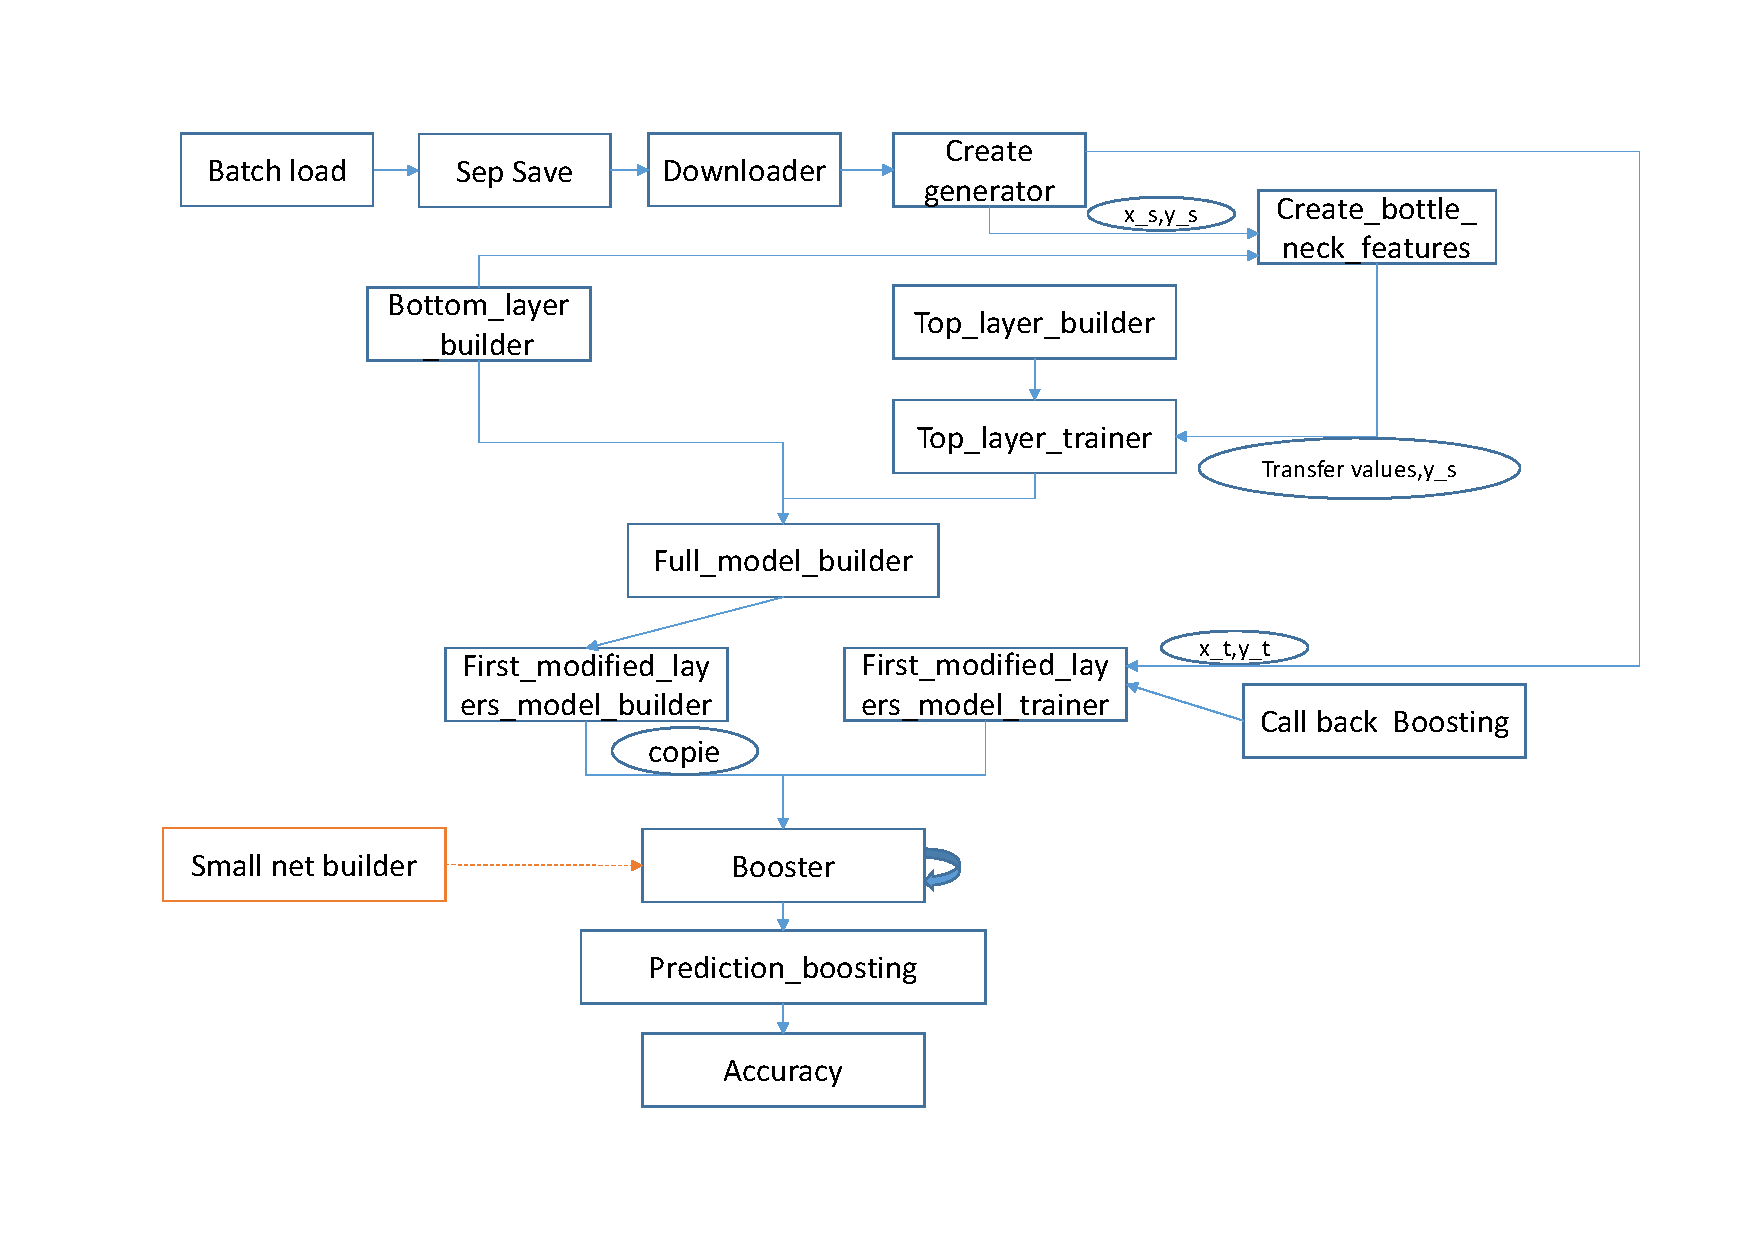
\includegraphics[width=\textwidth]{figTot.pdf}
    \caption{schema du programme}
    \label{figTot}
  \end{figure}

\end{appendices}

\end{document}
